\section{Geometry-dependent collapse}

Perturbations with the same initial defector count and resource deficit need not have the same probability of collapse. A dispersed perturbation creates more cooperator--defector contacts than a compact patch, altering the opportunities for early growth. Figures~\ref{fig:regimes} and \ref{fig:phase} show that this geometric distinction is most consequential near the crossover between recovery and persistent depletion. At stronger diffusion, the collapse probability changes rapidly with the defector payoff $b$; at weaker diffusion, a substantial fraction of trajectories remains unresolved within the observation window.


\begin{figure*}[tp]
\centering
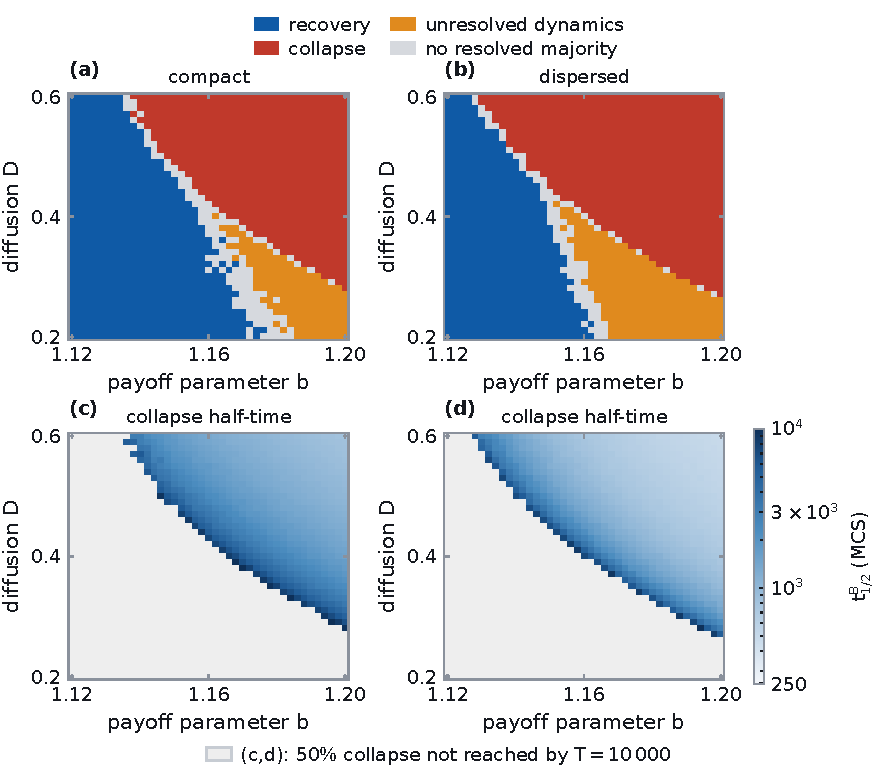
\includegraphics[width=0.85\textwidth]{fig00_dynamical_regimes.pdf}
\caption{Finite-time outcomes and collapse times for compact and dispersed perturbations ($L=48$, $m=16$, $T=10\,000$ MCS). (a,b) Parameter regions in which recovery ($A$), persistent depletion ($B$), or unresolved evolution ($U$) has a statistically resolved majority; gray cells have no resolved majority, as defined in Supplemental Material, Sec.~\ref{sm-sec:checks}. (c,d) First time $t_{1/2}^{B}$ at which 50\% of the full 64-trajectory ensemble has recorded event $B$; gray indicates that this level is not reached within the observation window. Each panel shows the measured $\PhaseBPoints\times\PhaseDPoints$ parameter grid without interpolation. All other parameters take their reference values.}
\label{fig:regimes}
\end{figure*}


The time required for half of the initial ensemble to confirm collapse is
\begin{equation}
\label{eq:collapse_half_time}
t_{1/2}^{B}=\inf\{t:\widehat P_B(t)\ge1/2\}.
\end{equation}
The dispersed preparation reaches a 50\% collapse probability in part of the parameter plane where the compact preparation does not. A low measured collapse probability, however, does not necessarily imply recovery: the disturbance may have disappeared, or it may remain active without satisfying either stopping criterion. The unresolved category must therefore be shown explicitly when interpreting finite-time regime maps.


\begin{figure*}[tp]
\centering
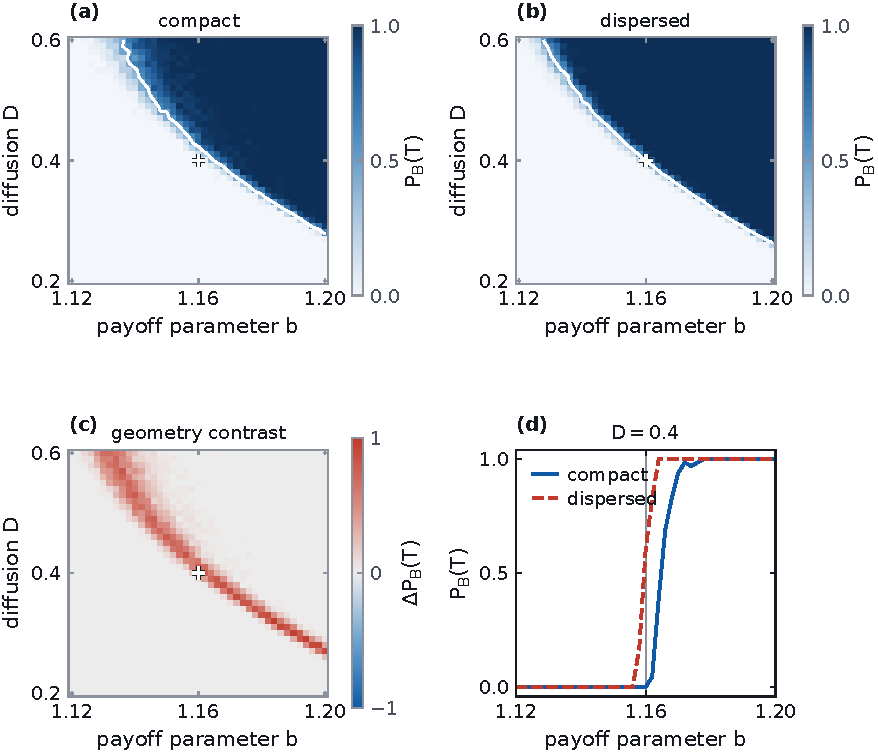
\includegraphics[width=0.85\textwidth]{fig01_phase.pdf}
\caption{Collapse-probability contrast between perturbation geometries. (a,b) Finite-time collapse probabilities for compact and dispersed seeds in the $(b,D)$ plane. (c) Difference $P_B^{\rm dispersed}(T)-P_B^{\rm compact}(T)$. (d) Cross section at $D=0.4$. Each grid point represents 64 independent realizations per geometry at $T=10\,000$ MCS. Cell colors show measured estimates without image interpolation; white half-probability contours are visual guides obtained by interpolation. Crosses indicate the reference parameters, and lines in (d) connect measured values.}
\label{fig:phase}
\end{figure*}


Figure~\ref{fig:phase} makes the displacement of the crossover more apparent. Dispersed seeds reach comparable collapse probabilities at lower values of $b$ than compact seeds, and increasing diffusion shifts both crossovers in the same direction. Their contrast is concentrated near the crossover rather than spread uniformly across parameter space. The larger separation in collapse probabilities is also present in the longer observation window discussed below. Because unresolved trajectories are retained, the observed ordering does not depend on classifying them as either recovery or collapse. These results establish a finite-time, geometry-dependent difference in collapse risk; they do not by themselves establish an asymptotic phase transition, which would require the size and time dependence used to identify absorbing-state transitions \cite{hinrichsen2000absorbing,marro1999nonequilibrium}. Quantitative estimates and their uncertainties are given in Sec.~\ref{sm-sec:checks} of the Supplemental Material.
